\chapter{Evaluation}


%In this chapter you should describe the previous (if possible) and final experiments performed on the implementation.

%Every single experiment should be explained individually, providing to the reader information about the meaning of the experiment, the expected (theoretical) results, the final results, the comparison between them and others (if possible) and the conclusions. 

%Each experiment should include a description, covering (when possible) the following information:
%\begin{itemize}
%	\item Significant physical features (obstacles present on the environment, human presence, temperature, humidity, possible noise sources, computational speed of the machine, etc.)
%	\item The precise location of the experiment (latitude and longitude, room number or citation to a description of the used laboratory).
%	\item Sampling design (variable(s) measured, transformation performed to the data, samples collected, replication, comparative with a Ground Truth system, collecting data protocol).
%	\item Analysis design (how the data are processed, statistical procedures used, statistical level to determine significance).
%\end{itemize}
%The provided information should be sufficient to allow other scientists to repeat your experiment in the same conditions. Thus, the use of standard and well-known equipment could only be represented by a simple sentence, but the non-standard equipment should be described in detail, citing the source (vendor) and most important characteristics.

%To write it, try to use the third person when describing the experiments and results. Avoid to use first person. Past tense should be the dominant conjugation (the work is done and was performed in the past).

%Note: Graphics represent really well data, use them! (Matlab or Octave could be useful for that).
Simulation experiment were conducted using a multirobot simulation enviroment(Figure \ref{fig:gazebo_model}) Gazebo. As discussed in section \ref{sec:system_enviroment}, the map (Figure \ref{fig:exp_map}) is greated by SLAM \cite{slam}. The are important coordinates: D1-D17 represent doors; C1-C3 represent charging stations; P1-P10 represent points used as goal positions in experiments.
Followings are goals of experiments:

\begin{itemize}
	\item Evaluate the need of decition variables.
	\item Find the best weight combinations in cost functions.
%	\item Investigate how different weight combinations in cost functions affact the performance \cite{Shiqi}. 
\end{itemize}

\begin{figure}[htbp]
	\centering
	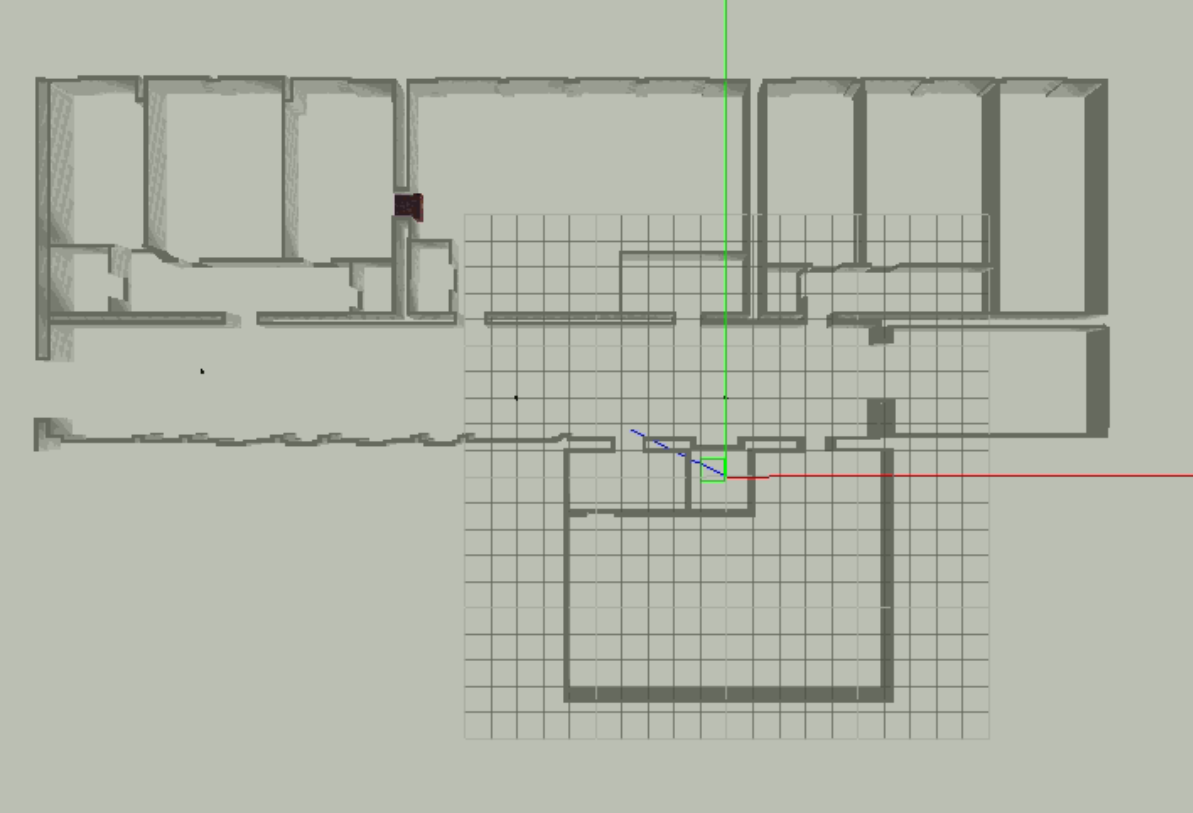
\includegraphics[width = 0.7\textwidth]{content/images/ch5/gazebo_model.png}
	\caption{Gazebo Simulation}
	\label{fig:gazebo_model}
\end{figure}

\begin{figure}[htbp]
    \centering
    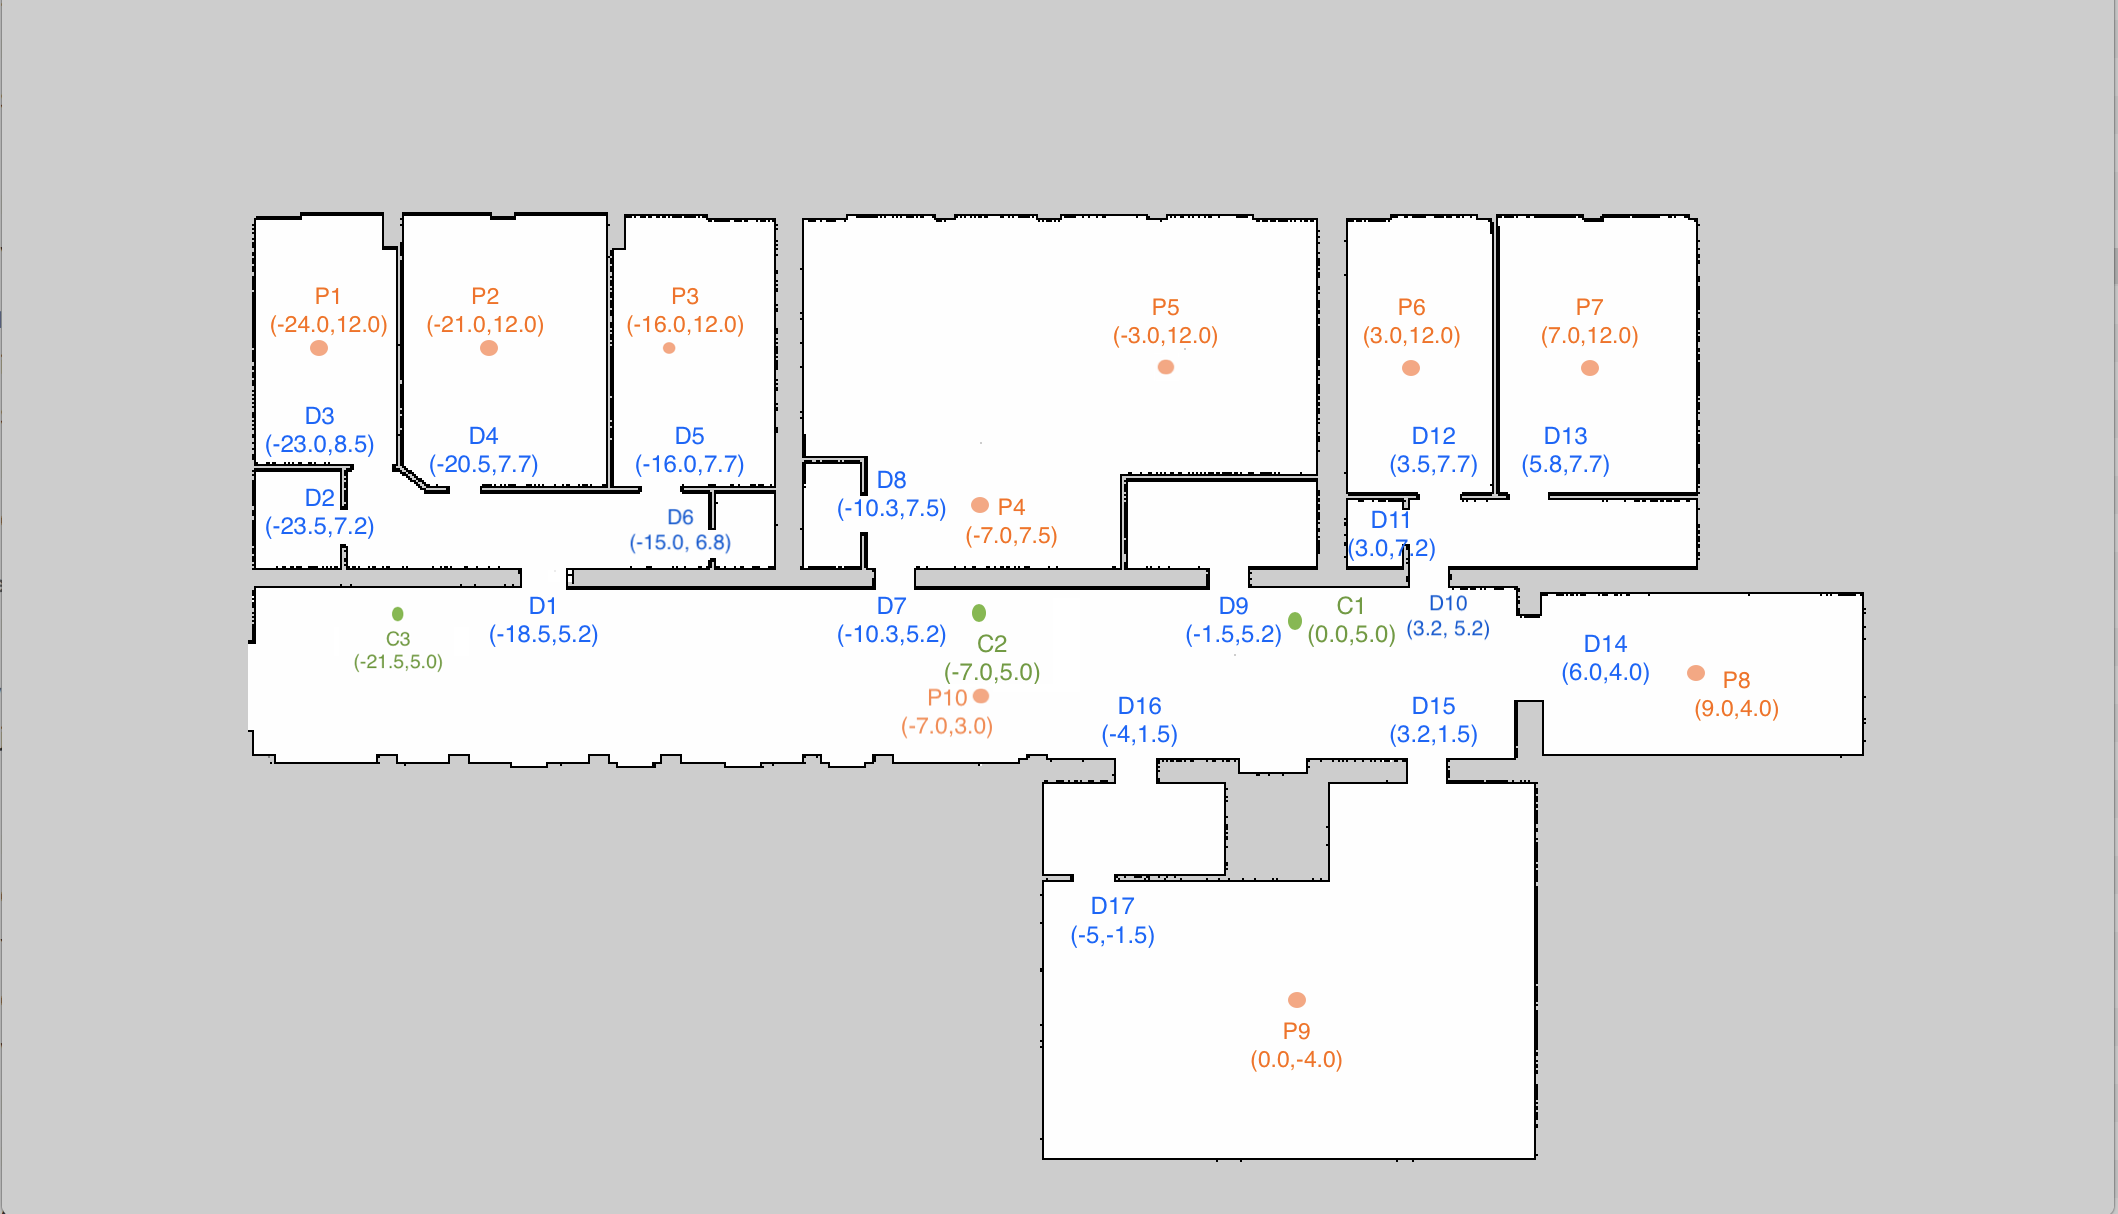
\includegraphics[width = 0.9\textwidth]{content/images/ch5/door_station_points.png}
    \caption{Experiment Map}
    \label{fig:exp_map}
\end{figure}

\section{Execute Task Evaluation}

\paragraph{Experiment precondition}
There are some preconditions for every experiment. When simulation started, robots moved to corresponding charging station and started charging. For example, robot 1 charged at charging staion 1, robot 2 charged at charging staion 2, robot 3 charged at charging staion 3(Figure \ref{fig:execute_task_experiment_timeline}). 
Once robot fully charged, the next experiment started, and 15 execute tasks are created. Especially, for each experiment, tasks with the same ID has the same start time and the same goal position. When all robot finished tasks, the experiment finished.
These rules ensure that robot would not only start at same initial points but also process same task and not shut down because of power exhaustion.

\begin{figure}[htbp]
    \centering
    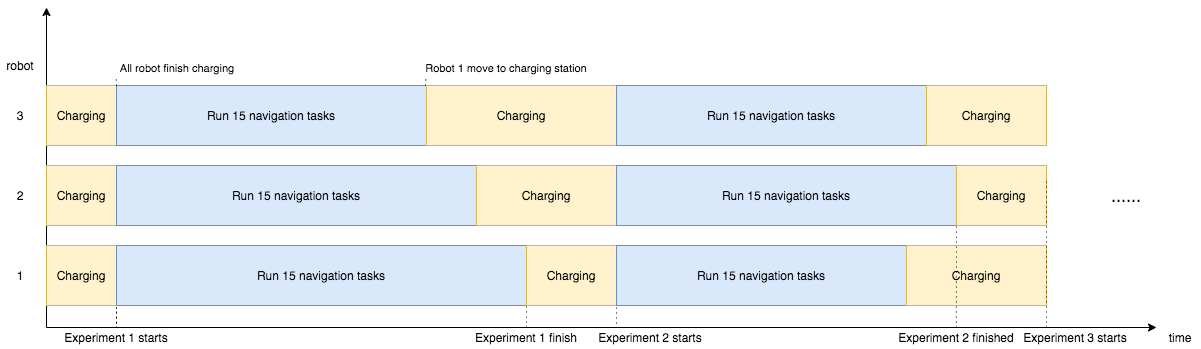
\includegraphics[width = 0.9\textwidth]{content/images/ch5/exe_exp_timeline.drawio.png}
    \caption{Execute Task Experiment Timeline}
    \label{fig:execute_task_experiment_timeline}
\end{figure}

\subsection{Experiment: Need of decision variables}
As discussed in Section \ref{sec:exe_task_allocation}, there are four decision variables: battery consumption, waiting time, product of door open possibility and priority. 
The first set of experiments evaluated the need of decition variables in cost function. 
The experiment result (Table \ref{tab:exp_decision_variables}) shows that the experiment 1 used the minimum time and all 15 task are completed.
The experiment with decision variables cost function with multiple decision variables has better performance than a cost function with single decition variable.

\begin{table}[htb]
\centering
\resizebox{\textwidth}{!}{
\begin{tabular}{|c|c|c|c|c|c|c|c|c|c|c|c|} 
\hline
&\multicolumn{4}{|c|}{Weight Combination} & \multirow{2}{*}{Experiment Duration}& \multicolumn{3}{|c|}{Task Statistic}\\
\cline{1-5}\cline{7-9}
Experiment ID	& 	 Battery Consumption & Waiting Time & Door Open Possibility	&  Priority & ~	& Total	 & Completed &	 Expired	 \\
\hline
1	& 1.00 &	 1.00 &	 -1.00&  -1.00&	 00:18:23 &	 15 &	 15 &	 0	 \\
\hline
2	& 1.00 &	 0.00 &	 0.00 &	 0.00 &	 00:17:23 &	 15 &	 7 &	 8	\\ 
\hline
3	& 0.00 &	 1.00 &	 0.00 &	 0.00 &	 00:18:56 &	 15 &	 15 &	 0	 \\
\hline
4	& 0.00 &	 0.00 &	 -1.00 & 0.00 &	 00:18:41 &	 15 &	 5 &	 10	\\
\hline	 
5	& 0.00 &	 0.00 &	 0.00 &	 -1.00&	 00:17:21 &	 15 &	  3 &	 12	 \\	 
\hline
\end{tabular}}
\caption{Runing execute task with single decision variable and multiple decision variables}
\label{tab:exp_decision_variables}
\end{table}

\subsection{Experiment: Find the best weight combinations}

The 


